\documentclass[12pt]{iopart}
\bibliographystyle{unsrt}
\usepackage{cite}
\usepackage[colorlinks, citecolor = blue, urlcolor = blue]{hyperref}
\usepackage{lineno}
\usepackage{longtable}
\usepackage{threeparttable}
\usepackage{threeparttablex}
\usepackage{enumitem}
\usepackage{lscape}
\usepackage{xcolor}
\usepackage{graphicx}
\usepackage[utf8]{inputenc}
\usepackage[T1]{fontenc}
\usepackage{pdfpages}
\usepackage{siunitx}




\begin{document}

\title[Draft - May 2023]{Validation of the code TDCRPy against the code TDCR17}
\author{Romain Coulon}
\address{Bureau International des Poids et Mesures, Pavillon de Breteuil, F-92312 S\`{e}vres Cedex, France.}


\section{Introduction}

The code TDCR17 was developed in Fortran by Philippe Cassette at the LNE-LNHB to calculate the efficiency of a TDCR system. It was used by the LNE-LNHB and other laboratories in key comparisons such as in the CCRI(II)-K2.H-3(2018). The BIPM developed the python code TDCRPy to estimating detection efficiency of TDCR measurement. The aim of this study is to test the BIPM code against the TDCR17 code for pure beta radionuclides planned to be in the scope of the ESIR.\\

\tableofcontents

\pagebreak
\section{Measurement data and results}
\subsection{$^{14}$C}

\begingroup
\footnotesize
\begin{longtable}[l]{| p{.08\textwidth} | p{.08\textwidth} |p{.15\textwidth} |p{.15\textwidth} |p{.10\textwidth} |} 
\caption{Measurement data and results - $kB = 0.008$ cm $\cdot$ MeV$^{-1}$}
\label{Table1} \\ 
\hline
\textbf{Source} & \textbf{$TDCR$} & \textbf{$\epsilon_{D}$ TDCR17} & \textbf{$\epsilon_{D}$ TDCRPy} & error \\
\endfirsthead
\multicolumn{5}{c}{... Continuation of Table 1.}\\ 
\hline
 \textbf{Source} & \textbf{$TDCR$} & \textbf{$\epsilon_{D}$ TDCR17} & \textbf{$\epsilon_{D}$ TDCRPy} & error \\   \hline 
\endhead
\hline
 1 & 0.9   &   85.37 \% &   91.09 \% &  +5.72 \% \\
 2 & 0.8   &   72.88 \% &   83.64 \% &  +10.76 \% \\
 3 & 0.7   &   61.22 \% &   76.31 \% &  +15.09 \% \\
 4 & 0.6   &   50.09 \% &   67.84 \% &  +17.75 \% \\
 5 & 0.5   &   39.35 \% &   58.83 \% &  +19.48 \% \\
 6 & 0.4   &   29.00 \% &   48.17 \% &  +19.17 \% \\
 7 & 0.3   &   19.19 \% &   35.90 \% &  +16.71 \% \\
\hline
\end{longtable} 
\endgroup

\begingroup
\footnotesize
\begin{longtable}[l]{| p{.08\textwidth} | p{.08\textwidth} | p{.15\textwidth} |p{.15\textwidth} |p{.10\textwidth} |} 
\caption{Measurement data and results - $kB = 0.01$ cm $\cdot$ MeV$^{-1}$}
\label{Table1} \\ 
\hline
\textbf{Source} & \textbf{$TDCR$} & \textbf{$\epsilon_{D}$ TDCR17} & \textbf{$\epsilon_{D}$ TDCRPy} & error \\ 
\endfirsthead
\multicolumn{5}{c}{... Continuation of Table 1.}\\ 
\hline
 \textbf{Source} & \textbf{$TDCR$} & \textbf{$\epsilon_{D}$ TDCR17} & \textbf{$\epsilon_{D}$ TDCRPy} & error \\   \hline 
\endhead
\hline
 1 &  0.9  & 85.17 \% &  91.12 \% &  +5.95 \% \\
 2 &  0.8  & 72.60 \% &  83.38 \% &  +10.78 \% \\
 3 &  0.7  & 60.92 \% &  75.86 \% &  +14.96 \% \\
 4 &  0.6  & 49.80 \% &  67.52 \% &  +17.72 \% \\
 5 &  0.5  & 39.09 \% &  58.31 \% &  +19.22 \% \\
 6 &  0.4  & 28.79 \% &  47.75 \% &  +18.96 \% \\
 7 &  0.3  & 19.03 \% &  35.43 \% &  +16.40 \% \\
\hline
\end{longtable} 
\endgroup

\begingroup
\footnotesize
\begin{longtable}[l]{| p{.08\textwidth} | p{.08\textwidth} |p{.15\textwidth} |p{.15\textwidth} |p{.10\textwidth} |} 
\caption{Measurement data and results - $kB = 0.012$ cm $\cdot$ MeV$^{-1}$}
\label{Table1} \\ 
\hline
\textbf{Source} & \textbf{$TDCR$} & \textbf{$\epsilon_{D}$ TDCR17} & \textbf{$\epsilon_{D}$ TDCRPy} & error \\ 
\endfirsthead
\multicolumn{5}{c}{... Continuation of Table 1.}\\ 
\hline
 \textbf{Source} & \textbf{$TDCR$} & \textbf{$\epsilon_{D}$ TDCR17} & \textbf{$\epsilon_{D}$ TDCRPy} & error \\   \hline 
\endhead
\hline
 1 & 0.9   &  84.98 \% &  90.80 \% & +5.82 \% \\
 2 & 0.8   &  72.35 \% &  83.20 \% & +10.85 \% \\
 3 & 0.7   &  60.65 \% &  75.53 \% & +14.88 \% \\
 4 & 0.6   &  49.53 \% &  67.37 \% & +17.84 \% \\
 5 & 0.5   &  38.85 \% &  57.88 \% & +18.03 \% \\
 6 & 0.4   &  28.60 \% &  47.35 \% & +18.75 \% \\
 7 & 0.3   &  18.89 \% &  34.67 \% & +15.78 \% \\
\hline
\end{longtable} 
\endgroup

At $TDCR = 0.8$, $\Delta \epsilon_D = |83.20 - 83.64| = 0.44 \%$ for $kB = [0.008, 0.012]$ cm/MeV. The difference between software is largely higher $\approx 11 \%$. There is a problem probably due to the beta spectrum evaluation. 


\pagebreak
\subsection{$^{63}$Ni}

\begingroup
\footnotesize
\begin{longtable}[l]{| p{.08\textwidth} | p{.08\textwidth} |p{.15\textwidth} |p{.15\textwidth} |p{.10\textwidth} |} 
\caption{Measurement data and results - $kB = 0.008$ cm $\cdot$ MeV$^{-1}$}
\label{Table1} \\ 
\hline
\textbf{Source} & \textbf{$TDCR$} & \textbf{$\epsilon_{D}$ TDCR17} & \textbf{$\epsilon_{D}$ TDCRPy} & error \\
\endfirsthead
\multicolumn{5}{c}{... Continuation of Table 1.}\\ 
\hline
 \textbf{Source} & \textbf{$TDCR$} & \textbf{$\epsilon_{D}$ TDCR17} & \textbf{$\epsilon_{D}$ TDCRPy} & error \\   \hline 
\endhead
\hline
 1 & 0.9   &   89.34 \% &   89.38 \% &  +0.04 \% \\
 2 & 0.8   &   79.86 \% &   79.79 \% &  -0.07 \% \\
 3 & 0.7   &   70.80 \% &   70.70 \% &  -0.10 \% \\
 4 & 0.6   &   61.68 \% &   61.28 \% &  -0.40 \% \\
 5 & 0.5   &   52.12 \% &   51.42 \% &  -0.70 \% \\
 6 & 0.4   &   41.78 \% &   41.01 \% &  -0.77 \% \\
 7 & 0.3   &   30.46 \% &   29.88 \% &  -0.58 \% \\
\hline
\end{longtable} 
\endgroup


\begingroup
\footnotesize
\begin{longtable}[l]{| p{.08\textwidth} | p{.08\textwidth} | p{.15\textwidth} |p{.15\textwidth} |p{.10\textwidth} |} 
\caption{Measurement data and results - $kB = 0.01$ cm $\cdot$ MeV$^{-1}$}
\label{Table1} \\ 
\hline
\textbf{Source} & \textbf{$TDCR$} & \textbf{$\epsilon_{D}$ TDCR17} & \textbf{$\epsilon_{D}$ TDCRPy} & error \\ 
\endfirsthead
\multicolumn{5}{c}{... Continuation of Table 1.}\\ 
\hline
 \textbf{Source} & \textbf{$TDCR$} & \textbf{$\epsilon_{D}$ TDCR17} & \textbf{$\epsilon_{D}$ TDCRPy} & error \\   \hline 
\endhead
\hline
 1 &  0.9  &  89.03 \% &   88.98 \% & -0.05 \% \\
 2 &  0.8  &  79.35 \% &   79.54 \% & +0.20 \% \\
 3 &  0.7  &  70.19 \% &   70.27 \% & +0.08 \% \\
 4 &  0.6  &  61.04 \% &   60.69 \% & -0.35 \% \\
 5 &  0.5  &  51.49 \% &   50.78 \% & -0.71 \% \\
 6 &  0.4  &  41.22 \% &   40.24 \% & -0.98 \% \\
 7 &  0.3  &  30.02 \% &   29.12 \% & -0.90 \% \\
\hline
\end{longtable} 
\endgroup

\begingroup
\footnotesize
\begin{longtable}[l]{| p{.08\textwidth} | p{.08\textwidth} |p{.15\textwidth} |p{.15\textwidth} |p{.10\textwidth} |} 
\caption{Measurement data and results - $kB = 0.012$ cm $\cdot$ MeV$^{-1}$}
\label{Table1} \\ 
\hline
\textbf{Source} & \textbf{$TDCR$} & \textbf{$\epsilon_{D}$ TDCR17} & \textbf{$\epsilon_{D}$ TDCRPy} & error \\ 
\endfirsthead
\multicolumn{5}{c}{... Continuation of Table 1.}\\ 
\hline
 \textbf{Source} & \textbf{$TDCR$} & \textbf{$\epsilon_{D}$ TDCR17} & \textbf{$\epsilon_{D}$ TDCRPy} & error \\   \hline 
\endhead
\hline
 1 & 0.9   &   88.75 \% &   88.81 \% & +0.06 \% \\
 2 & 0.8   &   78.91 \% &   79.07 \% & +0.16 \% \\
 3 & 0.7   &   69.66 \% &   69.76 \% & +0.10 \% \\
 4 & 0.6   &   60.47 \% &   60.27 \% & -0.20 \% \\
 5 & 0.5   &   50.94 \% &   50.30 \% & -0.64 \% \\
 6 & 0.4   &   40.73 \% &   39.81 \% & -0.92 \% \\
 7 & 0.3   &   29.63 \% &   28.78 \% & -0.85 \% \\
\hline
\end{longtable} 
\endgroup

At $TDCR = 0.8$, $\Delta \epsilon_D = |79.07 - 79.79| = 0.72 \%$ for $kB = [0.008, 0.012]$ cm/MeV. The difference between software is lower $\approx 0.2 \%$. 

\pagebreak
\subsection{$^{3}$H}

\begingroup
\footnotesize
\begin{longtable}[l]{| p{.08\textwidth} | p{.08\textwidth} |p{.15\textwidth} |p{.15\textwidth} |p{.10\textwidth} |} 
\caption{Measurement data and results - $kB = 0.008$ cm $\cdot$ MeV$^{-1}$}
\label{Table1} \\ 
\hline
\textbf{Source} & \textbf{$TDCR$} & \textbf{$\epsilon_{D}$ TDCR17} & \textbf{$\epsilon_{D}$ TDCRPy} & error \\
\endfirsthead
\multicolumn{5}{c}{... Continuation of Table 1.}\\ 
\hline
 \textbf{Source} & \textbf{$TDCR$} & \textbf{$\epsilon_{D}$ TDCR17} & \textbf{$\epsilon_{D}$ TDCRPy} & error \\   \hline 
\endhead
\hline
 1 & 0.9   &   90.42 \% &   90.73 \% &  +0.31 \% \\
 2 & 0.8   &   81.92 \% &   82.20 \% &  +0.28 \% \\
 3 & 0.7   &   73.51 \% &   73.66 \% &  +0.15 \% \\
 4 & 0.6   &   64.75 \% &   64.60 \% &  -0.10 \% \\
 5 & 0.5   &   55.25 \% &   54.79 \% &  -0.46 \% \\
 6 & 0.4   &   44.70 \% &   44.14 \% &  -0.56 \% \\
 7 & 0.3   &   32.87 \% &   32.51 \% &  -0.36 \% \\
\hline
\end{longtable} 
\endgroup

\begingroup
\footnotesize
\begin{longtable}[l]{| p{.08\textwidth} | p{.08\textwidth} | p{.15\textwidth} |p{.15\textwidth} |p{.10\textwidth} |} 
\caption{Measurement data and results - $kB = 0.01$ cm $\cdot$ MeV$^{-1}$}
\label{Table1} \\ 
\hline
\textbf{Source} & \textbf{$TDCR$} & \textbf{$\epsilon_{D}$ TDCR17} & \textbf{$\epsilon_{D}$ TDCRPy} & error \\ 
\endfirsthead
\multicolumn{5}{c}{... Continuation of Table 1.}\\ 
\hline
 \textbf{Source} & \textbf{$TDCR$} & \textbf{$\epsilon_{D}$ TDCR17} & \textbf{$\epsilon_{D}$ TDCRPy} & error \\   \hline 
\endhead
\hline
 1 &  0.9  &  90.17 \% &   90.58 \% &  +0.41 \% \\
 2 &  0.8  &  81.44 \% &   81.72 \% &  +0.28 \% \\
 3 &  0.7  &  72.88 \% &   73.07 \% &  +0.19 \% \\
 4 &  0.6  &  64.03 \% &   63.99 \% &  -0.04 \% \\
 5 &  0.5  &  54.51 \% &   54.37 \% &  -0.14 \% \\
 6 &  0.4  &  44.00 \% &   43.74 \% &  -0.26 \% \\
 7 &  0.3  &  32.29 \% &   31.96 \% &  -0.33 \% \\
\hline
\end{longtable} 
\endgroup

\begingroup
\footnotesize
\begin{longtable}[l]{| p{.08\textwidth} | p{.08\textwidth} |p{.15\textwidth} |p{.15\textwidth} |p{.10\textwidth} |} 
\caption{Measurement data and results - $kB = 0.012$ cm $\cdot$ MeV$^{-1}$}
\label{Table1} \\ 
\hline
\textbf{Source} & \textbf{$TDCR$} & \textbf{$\epsilon_{D}$ TDCR17} & \textbf{$\epsilon_{D}$ TDCRPy} & error \\ 
\endfirsthead
\multicolumn{5}{c}{... Continuation of Table 1.}\\ 
\hline
 \textbf{Source} & \textbf{$TDCR$} & \textbf{$\epsilon_{D}$ TDCR17} & \textbf{$\epsilon_{D}$ TDCRPy} & error \\   \hline 
\endhead
\hline
 1 & 0.9   &   89.96 \% &   90.43 \% & +0.47 \% \\
 2 & 0.8   &   81.04 \% &   81.34 \% & +0.30 \% \\
 3 & 0.7   &   72.34 \% &   72.55 \% & +0.21 \% \\
 4 & 0.6   &   63.42 \% &   63.61 \% & +0.19 \% \\
 5 & 0.5   &   53.88 \% &   53.69 \% & -0.19 \% \\
 6 & 0.4   &   43.41 \% &   42.77 \% & -0.64 \% \\
 7 & 0.3   &   31.80 \% &   31.12 \% & -0.68 \% \\
\hline
\end{longtable} 
\endgroup

At $TDCR = 0.7$, $\Delta \epsilon_D = |72.55 - 73.66| = 1.11 \%$ for $kB = [0.008, 0.012]$ cm/MeV. The difference between software is lower $\approx 0.2 \%$ . 

\pagebreak
\subsection{$^{35}$S}

\begingroup
\footnotesize
\begin{longtable}[l]{| p{.08\textwidth} | p{.08\textwidth} |p{.15\textwidth} |p{.15\textwidth} |p{.10\textwidth} |} 
\caption{Measurement data and results - $kB = 0.008$ cm $\cdot$ MeV$^{-1}$}
\label{Table1} \\ 
\hline
\textbf{Source} & \textbf{$TDCR$} & \textbf{$\epsilon_{D}$ TDCR17} & \textbf{$\epsilon_{D}$ TDCRPy} & error \\
\endfirsthead
\multicolumn{5}{c}{... Continuation of Table 1.}\\ 
\hline
 \textbf{Source} & \textbf{$TDCR$} & \textbf{$\epsilon_{D}$ TDCR17} & \textbf{$\epsilon_{D}$ TDCRPy} & error \\   \hline 
\endhead
\hline
 1 & 0.9   &   90.34 \% &   89.85 \% &  -0.49 \% \\
 2 & 0.8   &   82.01 \% &   81.64 \% &  -0.37 \% \\
 3 & 0.7   &   73.88 \% &   73.48 \% &  -0.40 \% \\
 4 & 0.6   &   65.37 \% &   64.78 \% &  -0.59 \% \\
 5 & 0.5   &   56.07 \% &   55.07 \% &  -1.00 \% \\
 6 & 0.4   &   45.61 \% &   44.23 \% &  -1.38 \% \\
 7 & 0.3   &   33.73 \% &   32.66 \% &  -1.07 \% \\
\hline
\end{longtable} 
\endgroup


\begingroup
\footnotesize
\begin{longtable}[l]{| p{.08\textwidth} | p{.08\textwidth} | p{.15\textwidth} |p{.15\textwidth} |p{.10\textwidth} |} 
\caption{Measurement data and results - $kB = 0.01$ cm $\cdot$ MeV$^{-1}$}
\label{Table1} \\ 
\hline
\textbf{Source} & \textbf{$TDCR$} & \textbf{$\epsilon_{D}$ TDCR17} & \textbf{$\epsilon_{D}$ TDCRPy} & error \\ 
\endfirsthead
\multicolumn{5}{c}{... Continuation of Table 1.}\\ 
\hline
 \textbf{Source} & \textbf{$TDCR$} & \textbf{$\epsilon_{D}$ TDCR17} & \textbf{$\epsilon_{D}$ TDCRPy} & error \\   \hline 
\endhead
\hline
 1 &  0.9  &  90.08 \% &   89.74 \% &  -0.34 \% \\
 2 &  0.8  &  81.65 \% &   81.28 \% &  -0.37 \% \\
 3 &  0.7  &  73.47 \% &   73.07 \% &  -0.40 \% \\
 4 &  0.6  &  64.95 \% &   64.36 \% &  -0.59 \% \\
 5 &  0.5  &  55.67 \% &   54.78 \% &  -0.89 \% \\
 6 &  0.4  &  45.25 \% &   44.19 \% &  -1.06 \% \\
 7 &  0.3  &  33.44 \% &   32.84 \% &  -0.60 \% \\
\hline
\end{longtable} 
\endgroup

\begingroup
\footnotesize
\begin{longtable}[l]{| p{.08\textwidth} | p{.08\textwidth} |p{.15\textwidth} |p{.15\textwidth} |p{.10\textwidth} |} 
\caption{Measurement data and results - $kB = 0.012$ cm $\cdot$ MeV$^{-1}$}
\label{Table1} \\ 
\hline
\textbf{Source} & \textbf{$TDCR$} & \textbf{$\epsilon_{D}$ TDCR17} & \textbf{$\epsilon_{D}$ TDCRPy} & error \\ 
\endfirsthead
\multicolumn{5}{c}{... Continuation of Table 1.}\\ 
\hline
 \textbf{Source} & \textbf{$TDCR$} & \textbf{$\epsilon_{D}$ TDCR17} & \textbf{$\epsilon_{D}$ TDCRPy} & error \\   \hline 
\endhead
\hline
 1 & 0.9   &   89.86 \% &   89.40 \% &  -0.46 \% \\
 2 & 0.8   &   81.33 \% &   80.87 \% &  -0.46 \% \\
 3 & 0.7   &   73.10 \% &   72.42 \% &  -0.68 \% \\
 4 & 0.6   &   64.57 \% &   63.84 \% &  -0.73 \% \\
 5 & 0.5   &   55.30 \% &   54.27 \% &  -1.03 \% \\
 6 & 0.4   &   44.92 \% &   43.99 \% &  -0.93 \% \\
 7 & 0.3   &   33.18 \% &   32.43 \% &  -0.75 \% \\
\hline
\end{longtable} 
\endgroup

At $TDCR = 0.8$, $\Delta \epsilon_D = |80.87 - 81.64| = 0.77 \%$ for $kB = [0.008, 0.012]$ cm/MeV. The difference between software is lower $\approx 0.4 \%$ . 


\pagebreak
\subsection{$^{U}$X}

\begingroup
\footnotesize
\begin{longtable}[l]{| p{.08\textwidth} | p{.08\textwidth} |p{.15\textwidth} |p{.15\textwidth} |p{.10\textwidth} |} 
\caption{Measurement data and results - $kB = 0.008$ cm $\cdot$ MeV$^{-1}$}
\label{Table1} \\ 
\hline
\textbf{Source} & \textbf{$TDCR$} & \textbf{$\epsilon_{D}$ TDCR17} & \textbf{$\epsilon_{D}$ TDCRPy} & error \\
\endfirsthead
\multicolumn{5}{c}{... Continuation of Table 1.}\\ 
\hline
 \textbf{Source} & \textbf{$TDCR$} & \textbf{$\epsilon_{D}$ TDCR17} & \textbf{$\epsilon_{D}$ TDCRPy} & error \\   \hline 
\endhead
\hline
 1 & 0.9   &    \% &    \% &   \% \\
 2 & 0.8   &    \% &    \% &   \% \\
 3 & 0.7   &    \% &    \% &   \% \\
 4 & 0.6   &    \% &    \% &   \% \\
 5 & 0.5   &    \% &    \% &   \% \\
 6 & 0.4   &    \% &    \% &   \% \\
 7 & 0.3   &    \% &    \% &   \% \\
\hline
\end{longtable} 
\endgroup


\begingroup
\footnotesize
\begin{longtable}[l]{| p{.08\textwidth} | p{.08\textwidth} | p{.15\textwidth} |p{.15\textwidth} |p{.10\textwidth} |} 
\caption{Measurement data and results - $kB = 0.01$ cm $\cdot$ MeV$^{-1}$}
\label{Table1} \\ 
\hline
\textbf{Source} & \textbf{$TDCR$} & \textbf{$\epsilon_{D}$ TDCR17} & \textbf{$\epsilon_{D}$ TDCRPy} & error \\ 
\endfirsthead
\multicolumn{5}{c}{... Continuation of Table 1.}\\ 
\hline
 \textbf{Source} & \textbf{$TDCR$} & \textbf{$\epsilon_{D}$ TDCR17} & \textbf{$\epsilon_{D}$ TDCRPy} & error \\   \hline 
\endhead
\hline
 1 &  0.9  &   \% &    \% &  \% \\
 2 &  0.8  &   \% &    \% &  \% \\
 3 &  0.7  &   \% &    \% &  \% \\
 4 &  0.6  &   \% &    \% &  \% \\
 5 &  0.5  &   \% &    \% &  \% \\
 6 &  0.4  &   \% &    \% &  \% \\
 7 &  0.3  &   \% &    \% &  \% \\
\hline
\end{longtable} 
\endgroup

\begingroup
\footnotesize
\begin{longtable}[l]{| p{.08\textwidth} | p{.08\textwidth} |p{.15\textwidth} |p{.15\textwidth} |p{.10\textwidth} |} 
\caption{Measurement data and results - $kB = 0.012$ cm $\cdot$ MeV$^{-1}$}
\label{Table1} \\ 
\hline
\textbf{Source} & \textbf{$TDCR$} & \textbf{$\epsilon_{D}$ TDCR17} & \textbf{$\epsilon_{D}$ TDCRPy} & error \\ 
\endfirsthead
\multicolumn{5}{c}{... Continuation of Table 1.}\\ 
\hline
 \textbf{Source} & \textbf{$TDCR$} & \textbf{$\epsilon_{D}$ TDCR17} & \textbf{$\epsilon_{D}$ TDCRPy} & error \\   \hline 
\endhead
\hline
 1 & 0.9   &    \% &    \% &  \% \\
 2 & 0.8   &    \% &    \% &  \% \\
 3 & 0.7   &    \% &    \% &  \% \\
 4 & 0.6   &    \% &    \% &  \% \\
 5 & 0.5   &    \% &    \% &  \% \\
 6 & 0.4   &    \% &    \% &  \% \\
 7 & 0.3   &    \% &    \% &  \% \\
\hline
\end{longtable} 
\endgroup

\pagebreak
\section{Spectra}

\begin{figure}[h!]
\centering
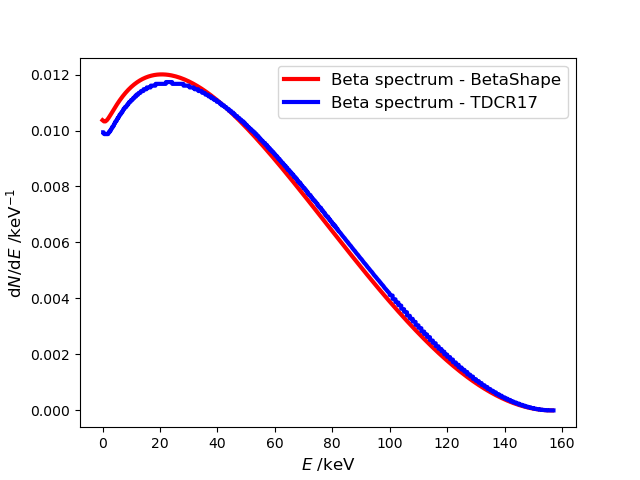
\includegraphics[scale=0.4]{../decayData/spectra/BetaSpectrum_C-14.png}
\caption{$\beta$ spectra of $^{14}$C from BetaShape (used in TDCRPy) and TDCR17}
\label{fig:C-14}
\end{figure}

\begin{figure}[h!]
\centering
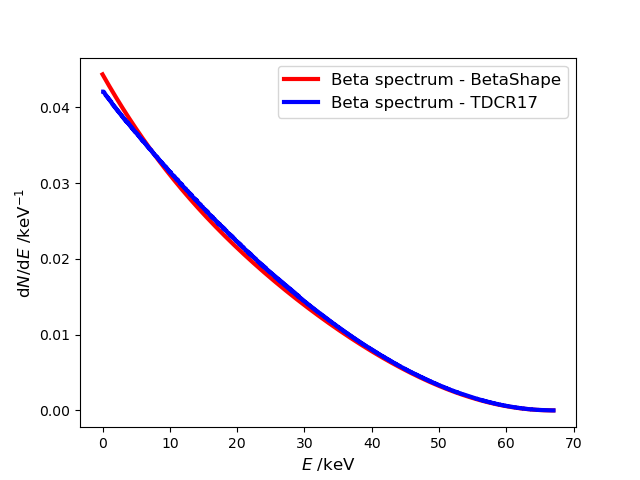
\includegraphics[scale=0.4]{../decayData/spectra/BetaSpectrum_Ni-63.png}
\caption{$\beta$ spectra of $^{63}$Ni from BetaShape (used in TDCRPy) and TDCR17}
\label{fig:Ni-63}
\end{figure}

\begin{figure}[h!]
\centering
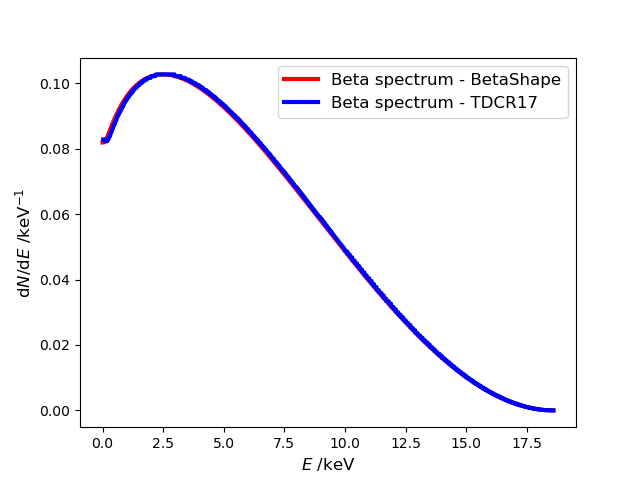
\includegraphics[scale=0.4]{../decayData/spectra/BetaSpectrum_H-3.png}
\caption{$\beta$ spectra of $^{3}$H from BetaShape (used in TDCRPy) and TDCR17}
\label{fig:H-3}
\end{figure}

\begin{figure}[h!]
\centering
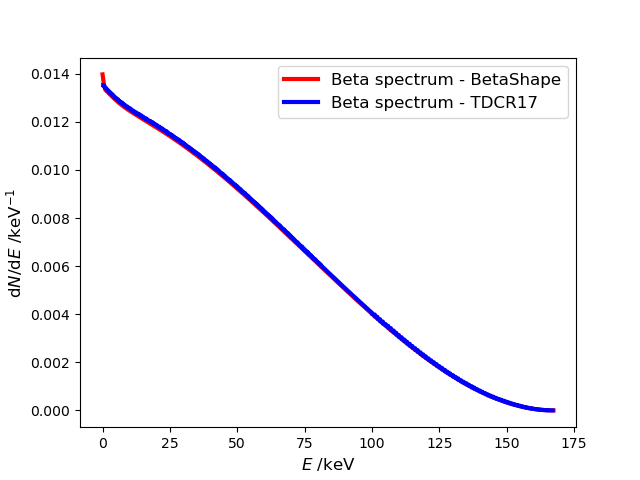
\includegraphics[scale=0.4]{../decayData/spectra/BetaSpectrum_S-35.png}
\caption{$\beta$ spectra of $^{35}$S from BetaShape (used in TDCRPy) and TDCR17}
\label{fig:S-35}
\end{figure}

\end{document}